\documentclass[11pt,a4paper]{article}
\usepackage[margin=2.5cm,bottom=2.7cm]{geometry}
\usepackage{fontspec}
\setmainfont{Noto Serif}
\setsansfont{Noto Sans}
\setmonofont{DejaVu Sans Mono}
\usepackage{setspace}
\onehalfspacing
\usepackage{microtype}
\usepackage{ragged2e}
\usepackage{graphicx}
\graphicspath{{../figures/}}
\usepackage{booktabs}
\usepackage{tabularx}
\usepackage{array}
\usepackage[table]{xcolor}
\usepackage{caption}
\usepackage{float}
\usepackage{hyperref}
\usepackage{fancyhdr}
\usepackage{titlesec}
\usepackage{tocloft}
\usepackage{url}
\usepackage{doi}
\usepackage{amsmath}
\usepackage{hanging}
\usepackage{listings}
\usepackage{enumitem}

\definecolor{bcuBlue}{HTML}{2479B9}
\definecolor{tableGray}{HTML}{F1F1F1}
\definecolor{codeBg}{HTML}{050505}
\definecolor{codeText}{HTML}{F5F5F5}
\definecolor{codeComment}{HTML}{9CA3AF}
\definecolor{codeKeyword}{HTML}{60A5FA}
\definecolor{codeString}{HTML}{FBBF24}

\hypersetup{
  colorlinks=true,
  linkcolor=black,
  urlcolor=bcuBlue,
  citecolor=black,
  pdfauthor={Student 26152255},
  pdftitle={Customer Segmentation in E-Commerce Using Purchasing Behaviour and K-Means Clustering}
}
\urlstyle{same}

\pagestyle{fancy}
\fancyhf{}
\fancyfoot[C]{\thepage}
\renewcommand{\headrulewidth}{0pt}
\renewcommand{\footrulewidth}{0pt}
\setlength{\footskip}{24pt}

\titleformat{\section}{\bfseries\large}{\thesection.}{0.55em}{}[\vspace{0.35em}{\color{bcuBlue}\titlerule[0.7pt]}]
\titleformat{\subsection}{\bfseries\normalsize}{\thesubsection}{0.55em}{}
\titlespacing*{\section}{0pt}{1.7em}{0.75em}
\titlespacing*{\subsection}{0pt}{1.2em}{0.45em}

\captionsetup{font=small,labelfont=bf,labelsep=period,justification=centering}
\renewcommand{\listfigurename}{Table of Figures}
\renewcommand{\listtablename}{Table of Tables}
\renewcommand{\cftsecfont}{\normalfont}
\renewcommand{\cftsecpagefont}{\normalfont}
\renewcommand{\cfttoctitlefont}{\bfseries\Large}
\renewcommand{\cftloftitlefont}{\bfseries\Large}
\renewcommand{\cftlottitlefont}{\bfseries\Large}
\setlength{\cftbeforesecskip}{0.25em}

\lstdefinestyle{pythonshot}{
  language=Python,
  backgroundcolor=\color{codeBg},
  basicstyle=\ttfamily\scriptsize\color{codeText},
  keywordstyle=\color{codeKeyword}\bfseries,
  commentstyle=\color{codeComment},
  stringstyle=\color{codeString},
  showstringspaces=false,
  breaklines=true,
  breakatwhitespace=false,
  frame=single,
  rulecolor=\color{black},
  xleftmargin=0.3em,
  xrightmargin=0.3em,
  aboveskip=0.6em,
  belowskip=0.6em,
  columns=fullflexible,
  keepspaces=true,
  tabsize=4
}
\lstdefinestyle{outputshot}{
  backgroundcolor=\color{codeBg},
  basicstyle=\ttfamily\scriptsize\color{codeText},
  showstringspaces=false,
  breaklines=true,
  frame=single,
  rulecolor=\color{black},
  columns=fullflexible
}

\newcommand{\GBP}{\textsterling}
\newcommand{\reporttitle}{Customer Segmentation in E-Commerce Using Purchasing Behaviour and K-Means Clustering}

\begin{document}
\justifying

% ---------- COVER: same information structure as supplied sample ----------
\thispagestyle{empty}
\begin{center}
{\Large\bfseries CMP 4294 -- Introduction to Artificial Intelligence\par}
\vspace{1.6cm}
{\LARGE\bfseries \reporttitle\par}
\vspace{1.9cm}

\begin{tabular}{>{\bfseries}rl}
Student Name: & \rule{7.0cm}{0.4pt}\\[0.55cm]
Student ID: & 26152255\\[0.55cm]
Module Leader: & \rule{7.0cm}{0.4pt}\\[0.55cm]
Date: & 5 October 2026\\
\end{tabular}

\vfill
{\small Birmingham City University\\
Sunway College\par}
\vspace{1.1cm}
{\color{bcuBlue}\rule{0.90\textwidth}{0.9pt}}
\end{center}
\clearpage

% ---------- TOC ----------
\setcounter{page}{2}
\tableofcontents
\clearpage

% ---------- FIGURES / TABLES ----------
\listoffigures
\vspace{1.0cm}
\listoftables
\clearpage

% ---------- ACKNOWLEDGEMENT ----------
\section*{Acknowledgement}
\addcontentsline{toc}{section}{Acknowledgement}
I would like to thank Birmingham City University, Sunway College and the module teaching team for providing the opportunity to complete this practical artificial-intelligence project. The assessment provided hands-on experience of preparing real e-commerce transaction data, applying a taught clustering method and interpreting the results critically. I also acknowledge the maintainers of the UCI Online Retail dataset and the open-source Python ecosystem, particularly pandas, NumPy, Matplotlib and scikit-learn, which made the reproducible analysis possible.
\clearpage

% ---------- ABSTRACT ----------
\section*{Abstract}
\addcontentsline{toc}{section}{Abstract}
Raw retail transaction records rarely reveal which customers behave alike. This report examines whether K-Means clustering can identify meaningful behavioural groups in e-commerce purchasing data. A reproducible 2,000-row subset of the UCI Online Retail dataset was used to build Recency, Frequency and Monetary (RFM) features for 141 customers. The features were standardised, and $K=2$ to $8$ was tested using inertia and silhouette analysis. $K=4$ was selected (silhouette 0.4714) and was stable across twenty initialisations, producing four segments: high-value loyal, frequent regular, occasional, and lapsed or low-engagement. A key limitation is that the customer-aware subset compresses the upper Frequency and Monetary tails.
\clearpage

% ---------- DOMAIN + PROBLEM ----------
\section{Domain Description}
E-commerce generates transaction-level data in which each row records a product purchased within an order. Individually, these rows describe what was sold; across many customers they carry behavioural information about how often people buy, how recently they bought and how much they spend. These patterns matter because customers differ widely in value and engagement, and retailers must decide where to focus limited retention and marketing effort. Customer segmentation groups customers who behave similarly, so that decisions can be framed around a few interpretable groups rather than thousands of individual histories. This report tests one data-driven way to form such groups without assuming that segmentation by itself improves sales.

\section{Problem Definition}
The research question is: \emph{can K-Means clustering identify meaningful customer groups from e-commerce purchasing behaviour so that the retailer can better understand high-value, regular, occasional and low-engagement customers?} Raw transaction records do not directly show which customers behave in similar ways. The task is descriptive rather than predictive: no outcome is forecast and no label is known in advance. The aim is to discover similar behavioural groups using one technique, K-Means clustering. Behaviour is summarised using Recency, Frequency and Monetary value, so each customer is represented by a small set of interpretable measures. Success is judged by whether the clusters are distinct, statistically supported and explainable in business terms.

% ---------- LITERATURE ----------
\section{Literature Review}
\subsection{K-Means Clustering}
K-Means is a centroid-based clustering method introduced by MacQueen (1967) and formalised through least-squares quantisation by Lloyd (1982). It partitions observations into $K$ groups by minimising within-cluster variance, assigning each point to the nearest centroid under Euclidean distance. Two properties are especially important here. First, distance is scale-sensitive, so variables measured in different units should be standardised before clustering (Pedregosa et al., 2011). Second, $K$ must be chosen in advance, which makes model selection a substantive decision rather than a default.

\subsection{RFM Customer Behaviour}
RFM is a long-established representation in which Recency, Frequency and Monetary value summarise purchasing behaviour (Hughes, 1994; Fader, Hardie and Lee, 2005). Using the same Online Retail data family, Chen, Sain and Guo (2012) demonstrated RFM-based customer segmentation for online retail, showing the direct relevance of behavioural grouping to this domain. Market-segmentation theory similarly frames customers as heterogeneous groups that may require different treatment (Wedel and Kamakura, 2000).

\subsection{Cluster Validation and Critical Interpretation}
Rousseeuw (1987) proposed the silhouette coefficient to assess how well a point fits its own cluster relative to the next closest cluster, providing a separation measure alongside inertia. K-Means nevertheless assumes roughly spherical and comparable clusters and offers no causal explanation: it describes similarity only. These properties shape both the method used here and the cautious interpretation of its outputs.
\clearpage

% ---------- DATASET ----------
\section{Dataset Description}
\subsection{Where the Data Comes From}
The source is the UCI Online Retail dataset (Chen, 2015), accessed through a Kaggle mirror (Kaggle, 2021). UCI records 541,909 transaction rows and licenses the dataset under CC BY 4.0. The project uses a reproducible 2,000-row customer-aware subset so the analysis remains manageable while retaining repeated purchasing histories.

\subsection{Dataset Characteristics}
\begin{table}[H]
\centering
\caption{Dataset characteristics.}\label{tab:characteristics}
\rowcolors{2}{tableGray}{white}
\begin{tabularx}{0.92\textwidth}{>{\bfseries}p{0.31\textwidth} X}
\rowcolor{bcuBlue}\color{white}Attribute & \color{white}Detail\\
Dataset name & Online Retail\\
Source & UCI Machine Learning Repository via Kaggle mirror\\
Original records & 541,909 transaction rows\\
Original features & 8\\
Project records & 2,000 transaction rows\\
Project customers & 141 unique CustomerID values\\
Data types & Identifier, text, numeric, DateTime, categorical\\
Main technique & K-Means clustering\\
Behavioural features & Recency, Frequency, Monetary value\\
\end{tabularx}
\end{table}

\subsection{CSV Preview and Notebook Access}
Table~\ref{tab:preview} shows actual rows from the submitted \texttt{ecommerce\_2000.csv}; these are not fabricated examples. The complete Python analysis is provided in the separately submitted Jupyter notebook. The notebook is structured to run sequentially in Google Colab or Jupyter and uses the exact CSV included in the submission ZIP. Repository-specific links are intentionally omitted from this anonymously marked report.

\begin{table}[H]
\centering
\caption{Preview of the submitted CSV dataset.}\label{tab:preview}
\scriptsize
\resizebox{\textwidth}{!}{
\begin{tabular}{llllllll}
\toprule
InvoiceNo & StockCode & Description & Quantity & InvoiceDate & UnitPrice & CustomerID & Country\\
\midrule
573152 & 23493 & VINTAGE DOILY TRAVEL SEWING KIT & 6 & 27-10-2011 20:16 & 1.95 & 17530 & United Kingdom\\
536595 & 20679 & EDWARDIAN PARASOL RED & 1 & 01-12-2010 17:24 & 5.95 & 13576 & United Kingdom\\
548315 & 84945 & MULTI COLOUR SILVER T-LIGHT HOLDER & 12 & 30-03-2011 12:34 & 0.85 & 16019 & United Kingdom\\
574086 & 23391 & I LOVE LONDON MINI BACKPACK & 4 & 03-11-2011 08:39 & 4.15 & 15651 & United Kingdom\\
568151 & 23409 & PHOTO FRAME LINEN AND LACE LARGE & 6 & 25-09-2011 11:39 & 3.75 & 17506 & United Kingdom\\
\bottomrule
\end{tabular}}
\end{table}
\clearpage

\subsection{Feature Descriptions}
\begin{table}[H]
\centering
\caption{Feature descriptions.}\label{tab:features}
\rowcolors{2}{tableGray}{white}
\begin{tabularx}{\textwidth}{>{\bfseries}p{0.19\textwidth} p{0.18\textwidth} X}
\rowcolor{bcuBlue}\color{white}Feature & \color{white}Type & \color{white}Description\\
InvoiceNo & Identifier & Order identifier; a C prefix marks a cancellation\\
StockCode & Identifier & Product code\\
Description & Text & Product description\\
Quantity & Numerical & Units purchased on the transaction line\\
InvoiceDate & DateTime & Date and time of the order\\
UnitPrice & Numerical & Price per unit in GBP\\
CustomerID & Identifier & Customer key used for customer-level RFM features\\
Country & Categorical & Customer country\\
\end{tabularx}
\end{table}

% ---------- PREPROCESSING ----------
\section{Data Pre-Processing}
\subsection{Loading and Inspecting the Dataset}
The notebook first loads the exact CSV included in the submission and inspects its shape, columns, data types, missing values, duplicates and obvious transaction-quality problems. The following code is taken directly from the submitted notebook.

\textbf{Code excerpt 1: loading and initial inspection}

\noindent The submitted notebook first checks for the CSV beside the notebook, then for the repository-style \texttt{data/} path. A verified remote fallback is used only when neither local copy is available. The excerpt below shows the current local-path logic used by the notebook without exposing repository-specific identity inside this anonymously marked report.

\begin{lstlisting}[style=pythonshot]
from pathlib import Path

root_csv = Path("ecommerce_2000.csv")
repo_csv = Path("data/ecommerce_2000.csv")

if root_csv.exists():
    DATA_PATH = root_csv
elif repo_csv.exists():
    DATA_PATH = repo_csv
else:
    # Colab fallback downloads the same verified project CSV
    # used for this report.
    DATA_PATH = root_csv

df = pd.read_csv(
    DATA_PATH,
    dtype={"CustomerID": "string"}
)

print("Shape:", df.shape)
print("Missing CustomerID:",
      int(df["CustomerID"].isna().sum()))
print("Duplicate rows:",
      int(df.duplicated().sum()))
print("Cancelled invoices:",
      int(df["InvoiceNo"].astype(str).str.startswith("C").sum()))
print("Rows with Quantity <= 0:",
      int((df["Quantity"] <= 0).sum()))
print("Rows with UnitPrice <= 0:",
      int((df["UnitPrice"] <= 0).sum()))
print("Unique customers:",
      int(df["CustomerID"].nunique()))
\end{lstlisting}

\begin{lstlisting}[style=outputshot]
Shape: (2000, 8)
Missing CustomerID: 0
Duplicate rows: 0
Cancelled invoices: 185
Rows with Quantity <= 0: 185
Rows with UnitPrice <= 0: 1
Unique customers: 141
\end{lstlisting}

\begin{figure}[H]
\centering
\begin{minipage}[c]{0.42\textwidth}
\centering
\fbox{\parbox[c][4.3cm][c]{0.88\linewidth}{
\centering
\textbf{Missing values: 0}\\[0.25cm]
No missing values were found across any of the eight submitted attributes.
}}
\end{minipage}
\hfill
\begin{minipage}[c]{0.54\textwidth}
\centering
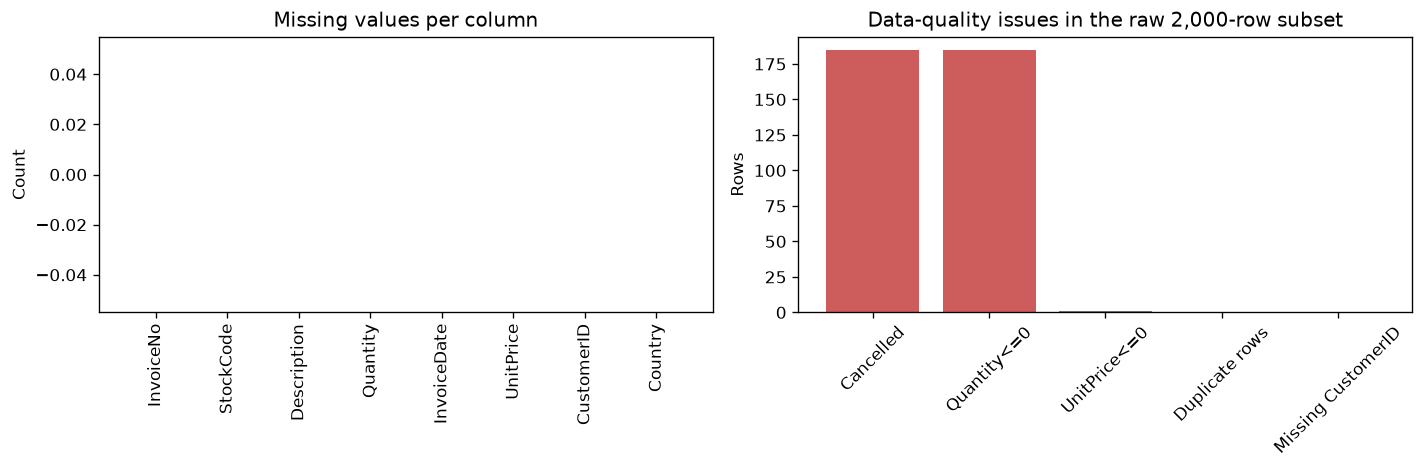
\includegraphics[width=\linewidth,trim=700 0 0 0,clip]{01_missing_values.png}
\end{minipage}
\caption{Data-quality issues in the 2,000-row project dataset. The left panel explicitly records zero missing values. The 185 cancelled invoices are the same 185 rows with non-positive quantity, so these two bars overlap and must not be added together.}\label{fig:quality}
\end{figure}
\clearpage

\subsection{Cleaning the Data and Creating Transaction Value}
Cancelled invoices were removed because they represent returns rather than purchases. In this project subset, the 185 cancelled invoices are the same 185 rows with non-positive quantity, so those two quality checks describe an overlapping set rather than 370 separate rows. Rows with non-positive quantity or unit price were excluded from spending analysis, exact duplicates were removed, and CustomerID was required for customer-level features. The resulting dataset contains 1,814 valid rows and 141 customers.

\textbf{Code excerpt 2: cleaning and TotalPrice}
\begin{lstlisting}[style=pythonshot]
rows_start = len(df)
data = df.copy()

# Remove cancelled invoices (returns)
data = data[
    ~data["InvoiceNo"].astype(str).str.startswith("C")
]

# Keep positive purchase quantities and prices
data = data[
    (data["Quantity"] > 0) &
    (data["UnitPrice"] > 0)
]

# Prevent double-counting exact repeated rows
data = data.drop_duplicates()

# Customer key is required for segmentation
data = data.dropna(subset=["CustomerID"])

data["InvoiceDate"] = pd.to_datetime(
    data["InvoiceDate"], format="%d-%m-%Y %H:%M"
)
data["TotalPrice"] = (
    data["Quantity"] * data["UnitPrice"]
)
\end{lstlisting}

\begin{lstlisting}[style=outputshot]
Initial project rows: 2000
After removing cancellations: 1815
After removing invalid quantity/price: 1814
After removing duplicates: 1814
Final cleaned rows: 1814
Unique customers after cleaning: 141
\end{lstlisting}

\begin{figure}[H]
\centering
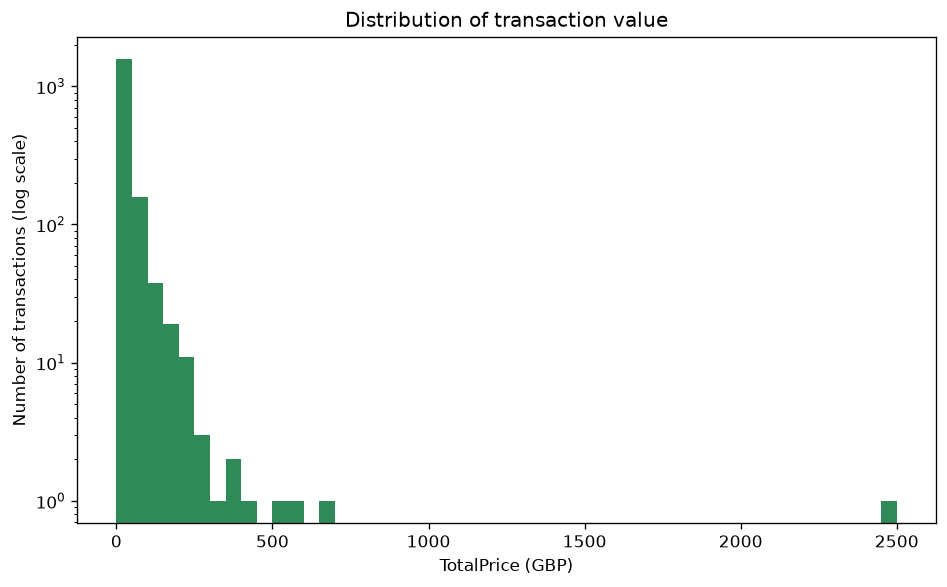
\includegraphics[width=0.78\textwidth]{02_transaction_distribution.png}
\caption{Distribution of cleaned transaction value.}\label{fig:transaction}
\end{figure}
\clearpage

\subsection{Creating RFM Features}
RFM converts line-level purchases into one row per customer. The notebook uses a reference date one day after the latest valid transaction. Recency is the number of days since the customer's latest purchase, Frequency is the number of distinct invoices, and Monetary is total cleaned spend.

\textbf{Code excerpt 3: customer-level RFM features}
\begin{lstlisting}[style=pythonshot]
snapshot = data["InvoiceDate"].max() + pd.Timedelta(days=1)

rfm = data.groupby("CustomerID").agg(
    Recency=(
        "InvoiceDate",
        lambda s: (snapshot - s.max()).days
    ),
    Frequency=("InvoiceNo", "nunique"),
    Monetary=("TotalPrice", "sum"),
)

print("Snapshot date:", snapshot.date())
print("Customers:", len(rfm))
rfm.describe().round(2)
\end{lstlisting}

\begin{table}[H]
\centering
\caption{RFM descriptive statistics.}\label{tab:rfmstats}
\rowcolors{2}{tableGray}{white}
\begin{tabular}{lrrr}
\rowcolor{bcuBlue}\color{white}Statistic & \color{white}Recency (days) & \color{white}Frequency (orders) & \color{white}Monetary (GBP)\\
Mean & 73.08 & 4.51 & 366.06\\
Median & 33.00 & 4.00 & 215.55\\
\end{tabular}
\end{table}

Three sampling constraints must be acknowledged: at most three line items per order, at most ten orders per customer, and exclusion of customers with more than thirty source orders. These choices preserve repeated histories under the 2,000-row project scope but compress the upper Frequency and Monetary tails.
\clearpage

% ---------- DESCRIPTIVE ANALYSIS ----------
\section{Descriptive Analysis Techniques}
\subsection{RFM Distributions}
Figure~\ref{fig:rfm} shows that Recency and Monetary are strongly right-skewed. Most customers have relatively recent activity and modest spend, while a small group of customers account for much larger monetary values. Frequency is bounded by the sampling design, which explains the visible upper limit at ten orders. These distributions justify scaling before Euclidean-distance clustering.

\begin{figure}[H]
\centering
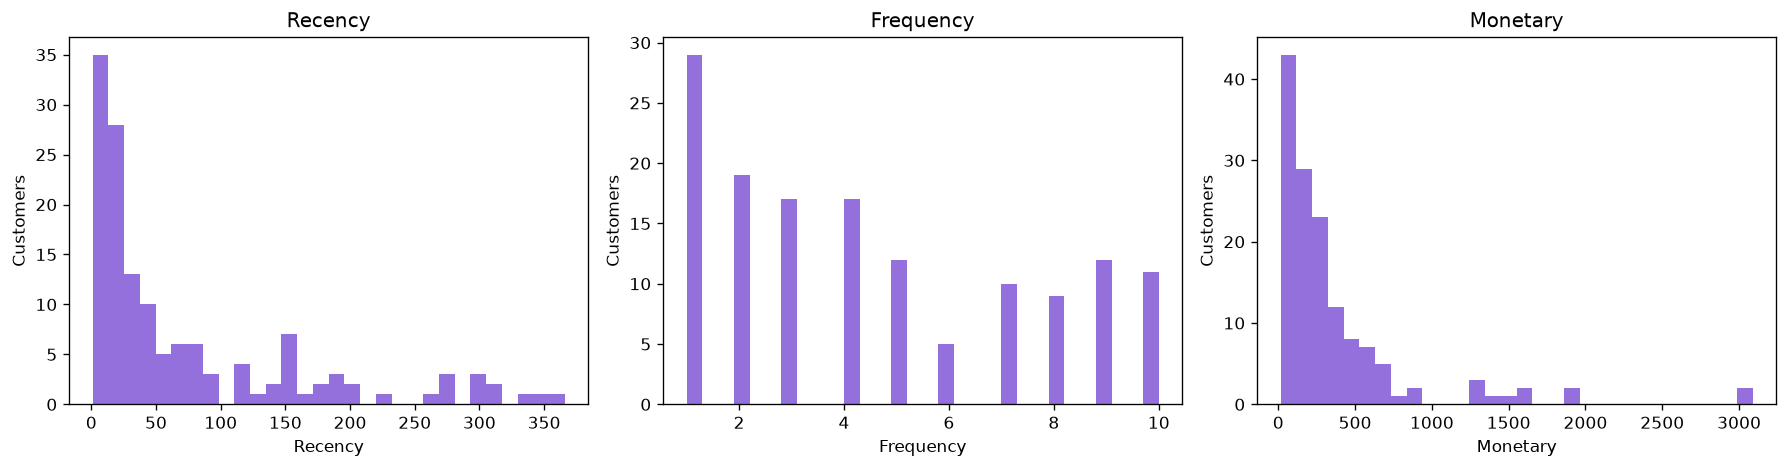
\includegraphics[width=\textwidth]{03_rfm_distributions.png}
\caption{RFM distributions for the 141 customers.}\label{fig:rfm}
\end{figure}

\subsection{Why Scaling Is Necessary}
Recency is measured in days, Frequency in orders and Monetary in pounds. Without standardisation, Monetary would dominate Euclidean distance simply because it has the largest numerical scale. The submitted notebook therefore transforms all three RFM features to comparable standardised values.

\textbf{Code excerpt 4: feature scaling}
\begin{lstlisting}[style=pythonshot]
scaler = StandardScaler()

X = scaler.fit_transform(
    rfm[["Recency", "Frequency", "Monetary"]].values
)

print("Scaled means:",
      np.round(X.mean(axis=0), 3))
print("Scaled stds :",
      np.round(X.std(axis=0), 3))
\end{lstlisting}

% ---------- EXPERIMENT ----------
\section{Experiments -- K-Means Clustering}
\subsection{Selecting the Number of Clusters}
The number of clusters was not chosen arbitrarily. Candidate solutions from $K=2$ through $8$ were fitted with a fixed random seed and \texttt{n\_init=10}. Inertia and silhouette score were recorded for each candidate.

\textbf{Code excerpt 5: testing K from 2 to 8}
\begin{lstlisting}[style=pythonshot]
k_values = list(range(2, 9))
inertias = []
silhouettes = []

for k in k_values:
    model = KMeans(
        n_clusters=k,
        random_state=RANDOM_STATE,
        n_init=10
    )
    labels = model.fit_predict(X)
    inertias.append(model.inertia_)
    silhouettes.append(
        silhouette_score(X, labels)
    )

results = pd.DataFrame({
    "K": k_values,
    "Inertia": np.round(inertias, 2),
    "Silhouette": np.round(silhouettes, 4)
})
results
\end{lstlisting}

\begin{table}[H]
\centering
\caption{Evaluation of candidate values of K.}\label{tab:k}
\rowcolors{2}{tableGray}{white}
\begin{tabular}{>{\bfseries}c rr}
\rowcolor{bcuBlue}\color{white}K & \color{white}Inertia & \color{white}Silhouette\\
2 & 247.11 & 0.4103\\
3 & 157.79 & 0.4329\\
4 & 91.01 & 0.4714\\
5 & 73.21 & 0.4625\\
6 & 56.88 & 0.4693\\
7 & 43.30 & 0.4270\\
8 & 38.53 & 0.3896\\
\end{tabular}
\end{table}
\clearpage

\subsection{Elbow and Silhouette Evidence}
Inertia falls sharply up to $K=4$ and then flattens, while the silhouette score reaches its maximum at $K=4$ (0.4714). The values for $K=4$, $5$ and $6$ are relatively close, so $K=4$ should be treated as the best-supported modelling choice for this sample rather than an absolute natural truth.

\begin{figure}[H]
\centering
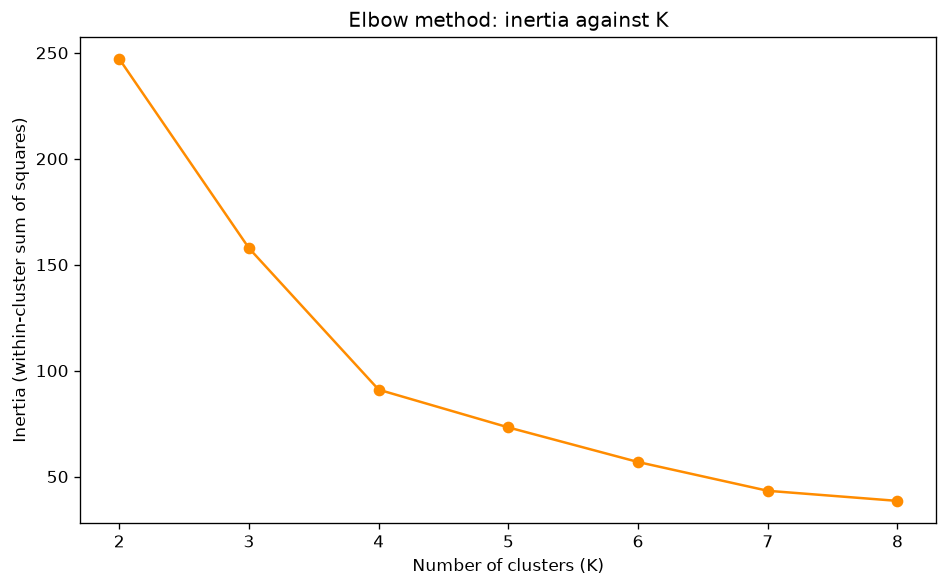
\includegraphics[width=0.76\textwidth]{04_elbow_method.png}
\caption{Elbow method: inertia against the number of clusters.}\label{fig:elbow}
\end{figure}

\begin{figure}[H]
\centering
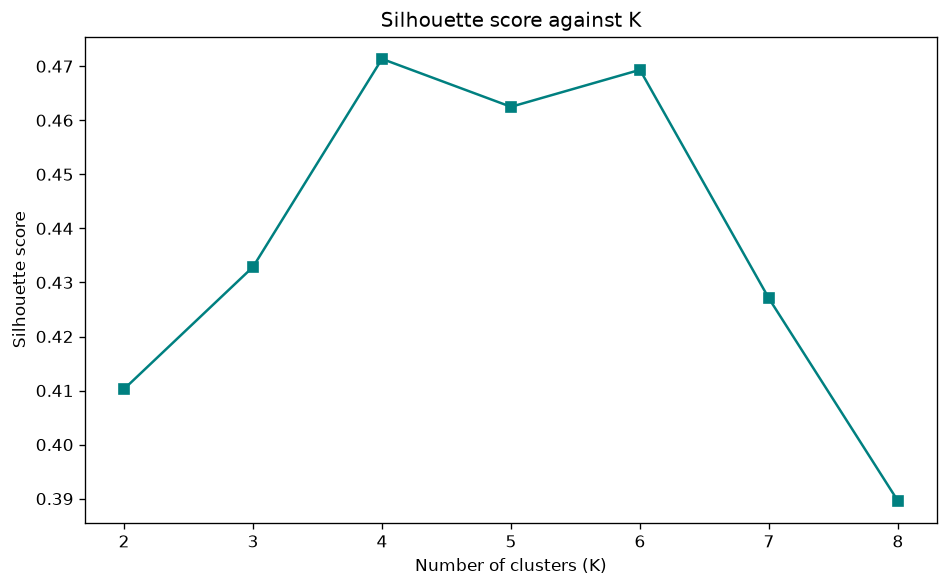
\includegraphics[width=0.76\textwidth]{05_silhouette_scores.png}
\caption{Silhouette score against the number of clusters.}\label{fig:sil}
\end{figure}
\clearpage

\subsection{Final K-Means Model and Cluster Profiles}
The final model uses four clusters, fixed \texttt{random\_state=42} and \texttt{n\_init=10}. Cluster profile statistics are then calculated directly from the customer-level RFM table.

\textbf{Code excerpt 6: final model and profiling}
\begin{lstlisting}[style=pythonshot]
final_k = 4

kmeans = KMeans(
    n_clusters=final_k,
    random_state=RANDOM_STATE,
    n_init=10
)
rfm["Cluster"] = kmeans.fit_predict(X)

print("Final inertia:",
      round(float(kmeans.inertia_), 2))
print("Final silhouette:",
      round(float(
          silhouette_score(X, rfm["Cluster"])
      ), 4))

profile = rfm.groupby("Cluster").agg(
    Customers=("Recency", "size"),
    Recency_mean=("Recency", "mean"),
    Recency_median=("Recency", "median"),
    Frequency_mean=("Frequency", "mean"),
    Frequency_median=("Frequency", "median"),
    Monetary_mean=("Monetary", "mean"),
    Monetary_median=("Monetary", "median"),
).round(2)
profile
\end{lstlisting}

\begin{table}[H]
\centering
\caption{Cluster profiles for the final K-Means model ($K=4$).}\label{tab:profiles}
\small
\rowcolors{2}{tableGray}{white}
\begin{tabularx}{\textwidth}{>{\bfseries}c c c c c X}
\rowcolor{bcuBlue}\color{white}Cluster & \color{white}Customers & \color{white}Recency & \color{white}Frequency & \color{white}Monetary (GBP) & \color{white}Interpretation\\
0 & 11 & 26.55 & 8.45 & 1,811.52 & High-value loyal\\
2 & 40 & 24.02 & 7.92 & 415.52 & Frequent regular\\
1 & 60 & 38.98 & 2.87 & 187.98 & Occasional\\
3 & 30 & 223.73 & 1.80 & 126.28 & Lapsed / low-engagement\\
\end{tabularx}
\end{table}
\clearpage

\subsection{Robustness to Initialisation}
Because K-Means can depend on initial centroid placement, the selected $K=4$ solution was re-fitted across random-state values 0--19 with \texttt{n\_init=10}. The silhouette score was 0.4714 in every run, the mean Adjusted Rand Index against the reference solution was 1.0, and only one cluster-size signature appeared (11, 30, 40, 60). This indicates stable initialisation for this project dataset, although it does not prove stability across different samples.

\textbf{Code excerpt 7: stability check}
\begin{lstlisting}[style=pythonshot]
reference = rfm["Cluster"].values
robust_sil = []
robust_ari = []

for seed in range(20):
    labels_seed = KMeans(
        n_clusters=final_k,
        random_state=seed,
        n_init=10
    ).fit_predict(X)

    robust_sil.append(
        silhouette_score(X, labels_seed)
    )
    robust_ari.append(
        adjusted_rand_score(reference, labels_seed)
    )

print("Silhouette mean:",
      round(np.mean(robust_sil), 4))
print("ARI mean:",
      round(np.mean(robust_ari), 4))
\end{lstlisting}

\begin{lstlisting}[style=outputshot]
Silhouette min / mean / max: 0.4714 / 0.4714 / 0.4714
Mean Adjusted Rand Index vs seed 42: 1.0000
Distinct cluster-size signatures: 1
\end{lstlisting}

% ---------- RESULTS ----------
\section{Analysis of Results and Conclusion}
\subsection{Cluster Results}
The four clusters differ clearly in the measured behaviour. Cluster 0 contains eleven customers who bought recently (mean Recency 26.55 days), most often (mean Frequency 8.45 orders) and with by far the highest spend (mean Monetary \GBP1,811.52); this is best described as a high-value loyal group. Cluster 2 (forty customers) is also recent and frequent (Recency 24.02; Frequency 7.92) but with moderate spend (\GBP415.52), suggesting a frequent regular group. Cluster 1 is larger (sixty customers) but purchases far less often (Frequency 2.87) and spends little (\GBP187.98), indicating an occasional group. Cluster 3 (thirty customers) is least recent (Recency 223.73 days), least frequent (1.80 orders) and lowest spend (\GBP126.28), consistent with a lapsed or low-engagement group. The numeric identifiers are arbitrary; the business labels are interpretations of the computed profiles rather than ground truth.

\begin{figure}[H]
\centering
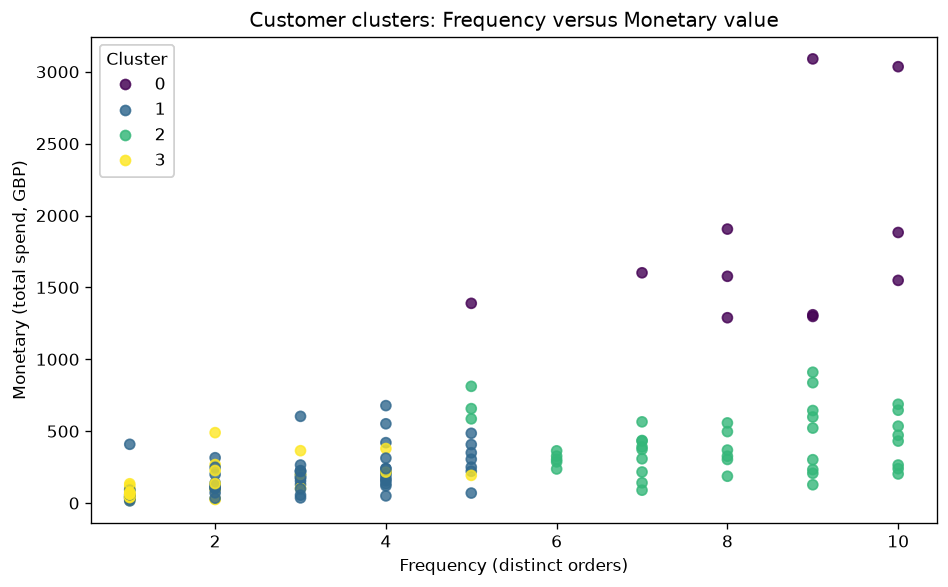
\includegraphics[width=0.77\textwidth]{06_customer_clusters.png}
\caption{Customer clusters: Frequency versus Monetary value.}\label{fig:scatter}
\end{figure}

\begin{figure}[H]
\centering
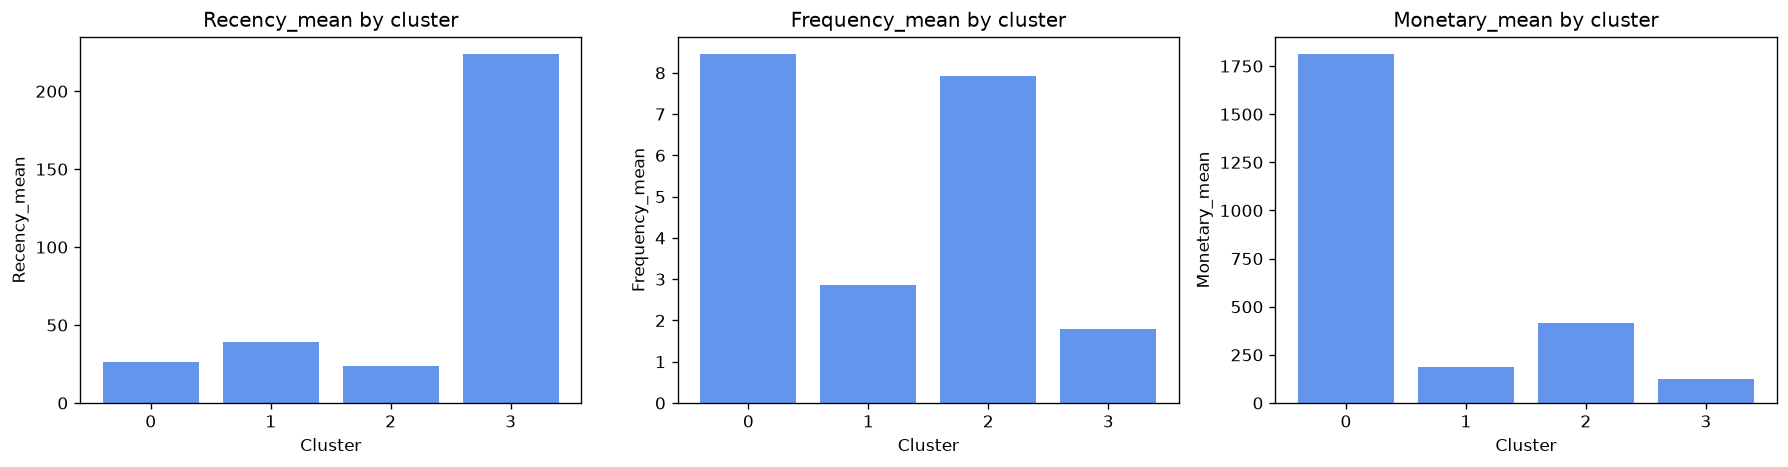
\includegraphics[width=\textwidth]{07_cluster_profiles.png}
\caption{Mean cluster profiles. Units are Recency in days, Frequency in distinct orders, and Monetary value in GBP.}\label{fig:profiles}
\end{figure}
\clearpage

\subsection{Business Interpretation}
Business implications follow from the observed profiles and are stated as possibilities rather than proven campaign effects. Retention or loyalty attention may be appropriate for the high-value loyal group, given its recent and frequent behaviour. The frequent regular group buys often at lower spend, so there may be potential to increase basket value. The occasional group is numerous but infrequent, suggesting an opportunity to encourage repeat purchases. The lapsed group could be a candidate for reactivation campaigns. These are hypotheses for later testing; the clustering data do not measure whether any intervention would increase revenue.

\subsection{Strengths and Limitations}
The analysis is reproducible and uses one taught method throughout. $K$ was selected using two complementary measures, the final clusters were profiled with interpretable customer statistics, and the robustness test shows the chosen solution is not sensitive to the tested initialisations. However, customer-aware sampling changes the original distribution. Capping line items and orders compresses the upper Frequency and Monetary tails, so the 141 customers cannot automatically represent the full retailer population. RFM also ignores product mix, margin, acquisition source, marketing exposure and website activity. K-Means assumes roughly spherical clusters, and $K$ selection remains a modelling decision. Most importantly, clustering identifies similarity, not causation.

\subsection{Conclusion}
The research question is supported for this project sample. K-Means identified four meaningful behavioural groupings from standardised RFM features: high-value loyal, frequent regular, occasional, and lapsed or low-engagement customers. $K=4$ produced the highest silhouette score (0.4714), aligned with the inertia elbow and remained stable across twenty tested initialisations. The segments offer a useful descriptive view of purchasing behaviour, but the sampling design and RFM limitations mean that the results should be interpreted cautiously rather than generalised automatically to the complete Online Retail population.

% ---------- REFERENCES ----------
\clearpage
\section*{References}
\addcontentsline{toc}{section}{References}
\begin{hangparas}{1.5em}{1}
Chen, D. (2015) \textit{Online Retail}. [dataset] UCI Machine Learning Repository. Available at: \url{https://doi.org/10.24432/C5BW33} [Accessed 5 October 2026].

Chen, D., Sain, S.L. and Guo, K. (2012) Data mining for the online retail industry: A case study of RFM model-based customer segmentation using data mining. \textit{Journal of Database Marketing \& Customer Strategy Management}, 19(3), pp. 197--208. \url{https://doi.org/10.1057/dbm.2012.17}.

Fader, P.S., Hardie, B.G.S. and Lee, K.L. (2005) RFM and CLV: Using iso-value curves for customer base analysis. \textit{Journal of Marketing Research}, 42(4), pp. 415--430. \url{https://doi.org/10.1509/jmkr.2005.42.4.415}.

Hughes, A.M. (1994) \textit{Strategic Database Marketing}. Chicago: Probus Publishing.

Kaggle (2021) \textit{Online Retail Business}. [dataset] Available at: \url{https://www.kaggle.com/datasets/umerkk12/online-retail-business} [Accessed 5 October 2026].

Lloyd, S.P. (1982) Least squares quantization in PCM. \textit{IEEE Transactions on Information Theory}, 28(2), pp. 129--137. \url{https://doi.org/10.1109/TIT.1982.1056489}.

MacQueen, J. (1967) Some methods for classification and analysis of multivariate observations. In: \textit{Proceedings of the Fifth Berkeley Symposium on Mathematical Statistics and Probability, Volume 1}. Berkeley: University of California Press, pp. 281--297.

Pedregosa, F. et al. (2011) Scikit-learn: Machine learning in Python. \textit{Journal of Machine Learning Research}, 12, pp. 2825--2830.

Rousseeuw, P.J. (1987) Silhouettes: A graphical aid to the interpretation and validation of cluster analysis. \textit{Journal of Computational and Applied Mathematics}, 20, pp. 53--65. \url{https://doi.org/10.1016/0377-0427(87)90125-7}.

Wedel, M. and Kamakura, W.A. (2000) \textit{Market Segmentation: Conceptual and Methodological Foundations}. 2nd edn. Boston: Kluwer Academic Publishers.
\end{hangparas}

\clearpage
\section*{Appendix A -- Reproducibility and Submitted Files}
\addcontentsline{toc}{section}{Appendix A -- Reproducibility and Submitted Files}
The submission package contains the Jupyter notebook and the exact CSV analysed in this report:

\begin{itemize}[leftmargin=2em]
\item Submitted Jupyter Notebook (\texttt{.ipynb})
\item \texttt{ecommerce\_2000.csv}
\end{itemize}

The notebook contains all Python used for loading, cleaning, RFM construction, scaling, K selection, K-Means fitting, cluster profiling, robustness testing and figure generation. It is designed to run sequentially in Google Colab or Jupyter without requiring Kaggle credentials. The 2,000-row project dataset was generated reproducibly from the full source file and is included with the submission.

\end{document}
